%%%%%%%%%%%%%%%%%%%%%%%%%%%%%%%%%%%%%%%%%%%%%%%%%%%%%%%%%%%%%%%%%%%%%%%%%%%%%%%%%%%%%%%%%%%%%%%%%%%%%%
%
%   Filename    : chapter_5.tex 
%
%   Description : This file will contain your Results and Analysis.
%                 
%%%%%%%%%%%%%%%%%%%%%%%%%%%%%%%%%%%%%%%%%%%%%%%%%%%%%%%%%%%%%%%%%%%%%%%%%%%%%%%%%%%%%%%%%%%%%%%%%%%%%%

\Section{Results and Analysis}
\label{sec:resultsandanalysis}

This chapter discusses the overall quality of the extracted relations. It also describes the results and the methodology in evaluating them.

\subsection{Methodology}
\label{sec:methodology}

In order to validate the quality of the extracted relations, they were used to generate stories in Picture Books. First, Picture Books was examined to determine which themes can be used. Then, the target relations extracted from the \textit{RAW} and \textit{MODIFIED} corpora were evaluated to see whether any of them can be easily inserted into the existing Picture Books ontology. Additional relations were manually added by the researcher for the target relations which did not have valid extractions from either corpora. Then, the Picture Books databases were manually updated with a select number of valid extractions, as well as the additional ones. 

\subsubsection{Examining the Picture Books Themes}
\label{sec:examinethemes}

Aside from checking the valid extractions that can be used for testing, the researcher also examined the themes of Picture Books. There are two motivations for this. First, the researcher would like to determine which among the themes can be used for testing. And secondly, he would like to map which target relation types can be tested for each theme selected.

After carefully tracing the ontology accesses and searches within the 15 different themes, five (5) were identified. Table \ref{tab:mapthemerel} shows the themes selected for testing with the mapped target relation types.

\begin{table}[H]   %t means place on top, replace with b if you want to place at the bottom
\centering
\caption{Mapping of Picture Books Themes with Target Relation Types} \vspace{0.25em}
\begin{tabular}{|p{5cm}|p{5cm}|} \hline
\textbf{Theme ID and Lesson} & \textbf{Mapped Target Relation Types} \\ \hline
THME0001: Take Bath			& usedFor \\ \hline
THME0003: Be Careful		& isA, capableOf, effectOf, propertyOf \\ \hline
THME0012: Be Honest			& isA, capableOf, effectOf, propertyOf \\ \hline
THME0005: Be Neat			& eventForGoalEvent \\ \hline
THME0015: Be Brave			& effectOfIsState \\ \hline
\end{tabular}
\label{tab:mapthemerel}
\end{table}  

After examination, only 7 target relation types were possible to be tested using the existing Picture Books themes.

\subsubsection{Grouping Target Relation Types}
\label{sec:grouprel}

Since only 7 target relation types can be tested by branching the existing ontology accesses and searches in the existing themes (See Section \ref{sec:examinethemes}), another group was created. This includes the 9 remaining target relation types which were not present in any of Picture Books' existing themes. A summary of the grouping is shown in Table \ref{tab:relgroups}.

\begin{table}[H]   %t means place on top, replace with b if you want to place at the bottom
\centering
\caption{Target Relation Type Groups} \vspace{0.25em}
\begin{tabular}{|p{5cm}|p{5cm}|} \hline
\textbf{Group A: Used in existing themes} & \textbf{Group B: Not used in existing themes} \\ \hline
isA, capableOf, propertyOf, effectOf, effectOfIsState, usedFor, eventForGoalEvent	& locationOf, partOf, madeOf, eventForGoalState, oftenNear, happens, hasRole, roleResponsibleFor, owns \\ \hline
\end{tabular}
\label{tab:relgroups}
\end{table}

\subsubsection*{Group A Relations}

For this group, 9 new lexicon entries and 12 new concepts were added into the database. The discrepancy was due to the words already existing in the lexicon but not as concepts to be used for ontology searches. Then, forty-one (41) new ontology entries were added to branch from existing ontology searches. Shown in Figure \ref{fig:altpath} is a sample alternative path created for this study. This is for author goal AUTH0026 of theme THME0003 (Be Careful).

\begin{figure}[h]                %-- use [t] to place figure at top, [b] to place at the bottom
   \centering                    %-- use this to center the figure
   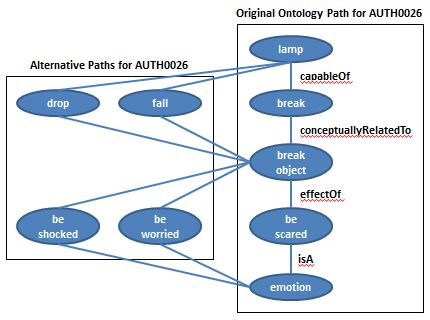
\includegraphics{altpath.jpg}      %-- include image file named as "sinag1.eps" 
   \caption{Alternative Path for AUTH0026}
    \label{fig:altpath}
\end{figure}

From the figure, there were 4 new concepts added and 8 new relations (2 \textit{IsA}, 2 \textit{ConceptuallyRelatedTo}, 2 \textit{EffectOf} and 2  \textit{CapableOf}). Though the relation \textit{ConceptuallyRelatedTo} is not really a target relation for this study, such entries were still created to maintain the path going to the last node (\textit{emotion}). 

However, as an exceptional case in this group of relations, the \textit{EffectOfIsState} relation was configured differently. Aside from the additional lexicon entries, concepts and ontology entries, 2 new author goals and 2 new story plot trackers were created. The new story plot trackers were then added as alternative Solutions to the theme THME0015 (Be Brave). This is all due to the difference in accessing the \textit{EffectOfIsState} in the author goal AUTH0056. Figure \ref{fig:altpatheffectofisstate} shows how the relation was accessed in the path. Instead of accessing the relation in the middle of the path, it was done at the end which was explicitly indicated in the definition of the author goal AUTH0056. This means there is no way to randomly select a new concept. 

\begin{figure}[h]                %-- use [t] to place figure at top, [b] to place at the bottom
   \centering                    %-- use this to center the figure
   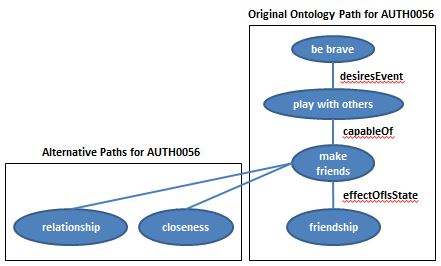
\includegraphics{altpatheffectofisstate.jpg}      %-- include image file named as "sinag1.eps" 
   \caption{Alternative Path for AUTH0056}
    \label{fig:altpatheffectofisstate}
\end{figure}

Appendix E shows all the additional entries in the Picture Books lexicon and ontology.

\subsubsection*{Group B Relations}

Because Group B relations did not exist in the current version of Picture Books' ontology, author goals were created to show the relations in the generated stories. 16 new lexicon entries and 20 new concepts were added into the database. Then, 27 new ontology entries were added. Finally, 9 new author goals were created and inserted as additional author goals of story plot tracker SPAT0004. 

For this group of relations, the theme THME0001 (Take Bath) was used. Each relation type had 2 representative sentences created and were included in the final story generated. None of the concepts and sentences were made coherent to the rest of the story. Appendix E shows all the additional entries in the Picture Books lexicon and ontology.

\subsubsection{Selected Relations}
\label{sec:selectedrelations}

Out of all the extracted relations from the \textit{RAW} and \textit{MODIFIED} corpora, only 6 relations were used and all of them are \textit{PartOf} relations. The rest of the relations used for testing were manually created. 

Group A needed extracted relations that are related to the themes selected as they are embedded in the ontology searches and accesses. But none of the extracted relations that fall under this group were coherent to any of the themes. \textit{EffectOfIsState} was also not extracted. Thus, it was decided to just create new relations that would be coherent to the rest of the stories. 

Group B, on the other hand, did not require the extracted relation to be coherent to the theme \textit{Take Bath} because that was not the intention. But because \textit{MadeOf} and \textit{OftenNear} were not extracted at all and \textit{EventForGoalState}, \textit{Happens}, \textit{HasRole}, \textit{Owns} and \textit{RoleResponsibleFor} did not have valid extractions, manual entries were also created.

\subsection{Extraction Analysis}
\label{sec:extractionanalysis}

There was a total of 13,871 unique relations extracted from the \textit{RAW} and \textit{MODIFIED} corpora. Tables \ref{tab:modifiedtotal} and \ref{tab:rawtotal} show the breakdown of numbers for each group of stories in each corpora.

\begin{table}[H]   %t means place on top, replace with b if you want to place at the bottom
\centering
\caption{Modified Corpus: Number of Unique and Redundant Relations Extracted} \vspace{0.25em}
\begin{tabular}{|p{4cm}|p{3cm}|p{3cm}|} \hline
\textbf{Story Group} & \textbf{Unique} & \textbf{Redundant} \\ \hline
Jumpstart & 729 & 206 \\ \hline
Winnie the Pooh & 436 & 137 \\ \hline
Topsy Tim & 747 & 341 \\ \hline
Little Life Lessons & 5260 & 2621 \\ \hline
\textbf{TOTAL} & \textbf{7172} & \textbf{3305} \\ \hline
\end{tabular}
\label{tab:modifiedtotal}
\end{table}

\begin{table}[H]   %t means place on top, replace with b if you want to place at the bottom
\centering
\caption{Raw Corpus: Number of Unique and Redundant Relations Extracted} \vspace{0.25em}
\begin{tabular}{|p{4cm}|p{3cm}|p{3cm}|} \hline
\textbf{Story Group} & \textbf{Unique} & \textbf{Redundant} \\ \hline
Jumpstart & 644 & 194 \\ \hline
Winnie the Pooh & 394 & 94 \\ \hline
Topsy Tim & 684 & 215 \\ \hline
Little Life Lessons & 4977 & 2017 \\ \hline
\textbf{TOTAL} & \textbf{6699} & \textbf{2520} \\ \hline
\end{tabular}
\label{tab:rawtotal}
\end{table}

From these numbers, it is evident that the \textit{Modified} corpus had 473 more relations extracted than the \textit{Raw} corpus. This suggests that the modifications done introduced new concepts, thus allowing the application to extract more unique relations. These modifications may have also introduced more redundant relations as the number increased by 785. This was even more than the increase in unique relations. 

In terms of relations, Table \ref{tab:reltotal} shows the breakdown of extracted relations per corpora. The delta after modification is also shown. 

\begin{table}[H]   %t means place on top, replace with b if you want to place at the bottom
\centering
\caption{Number of Relations Extracted per Corpus} \vspace{0.25em}
\begin{tabular}{|p{4.5cm}|p{2cm}|p{2cm}|p{2cm}|} \hline
\textbf{Relations} & \textbf{Raw} & \textbf{Modified} & \textbf{Delta} \\ \hline
IsA & 191 & 228 & 37 \\ \hline
PropertyOf & 2700 & 2857 & 157 \\ \hline
PartOf  & 71 & 84 & 13 \\ \hline
MadeOf & 0 & 0 & 0 \\ \hline
EventForGoalEvent & 481 & 580 & 99 \\ \hline
EventForGoalState & 31 & 37 & 6 \\ \hline
EffectOf & 1258 & 1196 & -62 \\ \hline
EffectOfIsState & 0 & 0 & 0 \\ \hline
CapableOf & 980 & 1193 & 213 \\ \hline
OftenNear & 0 & 0 & 0 \\ \hline
LocationOf & 136 & 137 & 1 \\ \hline
UsedFor & 228 & 232 & 4 \\ \hline
Happens & 38 & 34 & -4 \\ \hline
HasRole & 11 & 14 & 3 \\ \hline
RoleResponsibleFor & 11 & 13 & 2 \\ \hline
Owns & 562 & 565 & 3 \\ \hline
\end{tabular}
\label{tab:reltotal}
\end{table}

In a relational level, almost all relations experienced an increase in the number of extractions except for \textit{EffectOf} and \textit{Happens}. Again, although the delta is not significant in number, it suggests that the modifications avoided the extraction of possible relations. Here is an  extracted relation from the \textit{Raw} corpus that is not included as an extracted relation in the \textit{Modified} corpus:

\begin{verse}
\itshape
EffectOf(said,not forgive and forget)
\end{verse}

It was extracted from this passage from \textit{Forgive and Forget} of the \textit{Winnie the Pooh} story group:

\begin{verse}
\itshape
``Rabbit, I think Tigger is very sorry," Pooh said. ``Will you not forgive and forget?"
\end{verse}

This specific sentence was modified to this:

\begin{verse}
\itshape
Pooh thinks Tigger is very sorry. Pooh asks Rabbit if he can forgive and forget.
\end{verse}

In this example, the verb \textit{said} was removed after modification, thus avoiding the possibility of another relation being extracted. It seems that modifications, such as this, improved the result for the \textit{Modified} corpus because the relation is not really a valid and logical extraction. However, the possibility that valid extractions may also be omitted in the process cannot be discounted.

From the same table, it is important to note that the \textit{EffectOfIsState}, \textit{MadeOf} and \textit{OftenNear} relations had 0 extractions from either corpora. This seems to be caused by their high dependence on indicators unlike the rest of the relations.

In terms of extraction quality, there are some relations which may have been incorrectly extracted or which may not be extracted at all because of incorrect tags. For instance, this relation was extracted from the \textit{Jumpstart} story group:

\begin{verse}
\itshape
EffectOf(went on full speed,shocked)
\end{verse}

The extraction seems valid from first glance, but looking at its original passage may suggest otherwise. Shown below is the modified passage from \textit{Just in time}. Instead of \textit{EffectOf}, a better extraction could have been \textit{EffectOfIsState} since \textit{being shocked} is an implied state. 

\begin{verse}
\itshape
Frankie went on full speed.\\
Hopsalot was shocked.
\end{verse}

Other incorrect extractions were due to a different part-of-speech information tagged to the concept and the lack of additional semantic information.

Lastly, it is important to note that for event relations like \textit{EffectOf} and \textit{EventForGoalEvent}, the extracted relations seem to be longer and more specific because the extractor uses whole phrases as concepts. This may be different from the concepts of Picture Books that are more generalized. Here are some example extractions:

\begin{verse}
\itshape
EffectOf(looked at the map,checked the wind)\\
EffectOf(pours something into the volcano,stopped him)\\
EventForGoalEvent(called everyone,go to the ship)
\end{verse}

For a more detailed look in the extraction results, kindly refer to Appendix D.

\subsection{Story Analysis}
\label{sec:storyanalysis}

Overall, the new relations were used accordingly. They were randomly selected and used interchangeably with the original relations. But the sentences generated were fairly acceptable. There are cases wherein the sentence is grammatically incorrect. For example, here is an original story generated for the \textit{Be Careful} theme:

\begin{alltt}
\textbf{Edward the elephant learns to be careful.}

[1]  The morning was sunny.
[2]  Edward the elephant was in the dining room.
[3]  He played near breakable glass of water.
[4]  Daddy Sam told Edward to be careful.
[5]  Edward continued to play glass of water near.
\emph{\textbf{[6]  He broke it.}}
\emph{\textbf{[7]  Edward was scared.}}
[8]  He hid away from Daddy Sam.
\emph{\textbf{[9]  Daddy Sam saw that glass of water was broken.}}
[10] Daddy Sam called Edward.
[11] Daddy Sam told Edward that he should have obeyed.
[12] He felt sorry.
[13] Daddy Sam cleaned up glass of water.
[14] Edward helped Daddy Sam to clean up.
[15] Daddy Sam reminded Edward to be careful.
[16] Being careful is important.
[17] From that day onwards, Edward always was careful.
\end{alltt}

This used the original relations of Picture Books. The highlighted lines show the sentences where the changes should happen. Shown below is another story using the same characters and objects as the story above. This time, the highlighted sentences are using different concepts based on the new additions to the lexicon and ontology.

\begin{alltt}
\textbf{Edward the elephant learns to be careful.}

[1]  The afternoon was sunny.
[2]  Edward the elephant was in the dining room.
[3]  He played near breakable glass of water.
[4]  Mommy Edna told Edward to be careful.
[5]  Edward continued to play glass of water near.
\emph{\textbf{[6]  Edward fell it.}}
\emph{\textbf{[7]  Edward was worried.}}
[8]  He hid away from Mommy Edna.
\emph{\textbf{[9]  Mommy Edna saw that glass of water was cracked.}}
[10] Mommy Edna called Edward.
[11] Mommy Edna told Edward that he should have obeyed.
[12] Edward felt sorry.
[13] Mommy Edna cleaned up glass of water.
[14] Edward helped Mommy Edna to clean up.
[15] She reminded Edward to be careful.
[16] Being careful is important.
[17] From that day onwards, Edward always was careful.
\end{alltt}

In line 6, instead of the usual action \textit{broke}, the story now uses \textit{fell}. However, the new sentence should have been ``It fell" or ``The glass of water fell." Since the relation used here is \textit{CapableOf(lamp,fall)}, it also logical to note that the \textit{lamp} can be the agent of the action instead of always being the character. 

Another new story worth pointing out is this:

\begin{alltt}
\textbf{Edward the elephant learns to be honest.}

[1]  The morning was warm.
[2]  Edward the elephant was in the dining room.
[3]  He played near breakable glass of water.
\emph{\textbf{[4]  Edward fell glass of water.}}
[5]  He was worried.
[6]  Mommy Edna saw that glass of water was smashed.
[7]  Edward told Mommy Edna that Porky the pig broke glass of water.
[8]  He was sad.
[9]  Porky cried.
[10] Edward felt guilty.
\emph{\textbf{[11] Edward told Mommy Edna that he dropped glass of water.}}
[12] Mommy Edna told Edward that he should have been honest.
[13] He apologized to Mommy Edna.
[14] Edward apologized to Porky.
[15] Mommy Edna told Edward to be honest.
[16] Mommy Edna told Edward that being honest is good.
[17] From that day onwards, Edward always was honest.
\end{alltt}

In this story, highlighted are the sentences using the \textit{CapableOf} relations with \textit{lamp} as the parent concept, \textit{CapableOf(lamp,fall)} and \textit{CapableOf(lamp,drop)}. Though it is valid to use both, having them in just one story creates inconsistencies. In line 4, it was already mentioned that the glass of water fell. And since the word \textit{fell} was used, there is an implication of an accident which creates a different dimension to the story. Now in line 11, though Edward is already admitting his fault, he suddenly said \textit{dropped} instead of the initial \textit{fell}. This might create confusion as dropping something makes the act intentional whereas when it fell, Edward may or may not have caused the action. When the act \textit{fell} was used in line 4, it expected that the same act is confessed in line 11.

Lastly, there are a number of instances where incorrect relations are picked up by Picture Books in doing ontology accesses and searches. As a result, incorrect sentences are generated. For example, in the story \textit{Roy the chicken learns to take bath.} shown below, lines 9 and 10 are produced using the same relation, \textit{OftenNear}. They also have the same parent concept which is \textit{school}. Line 9 has a correct child concept but Line 10 does not. Instead of either \textit{clinic}, \textit{mall} or \textit{market}, it used \textit{generic}. After examining the ontology, \textit{generic} is the child concept when the relation is \textit{PropertyOf}. This shouldn't be the case. 

The reason why this happens is because Picture Books searches its ontology not by the name of the relation but by its category. In the ontology, both \textit{OftenNear} and \textit{PropertyOf} are under the category \textit{spatial}. This causes Picture Books to not only randomize among \textit{OftenNear} relations but also including the \textit{PropertyOf} relation.

\begin{alltt}
[1]  Toys were the bedroom.
[2]  Playing is the playground.
[3]  An oak had trunk.
[4]  A person had a toe.
[5]  A book had paper.
[6]  It had ink.
[7]  Playing is dirty.
[8]  It was healthy.
\emph{\textbf{[9]  The school was the market.}}
\emph{\textbf{[10] It was generic.}}
[11] Eating dinner is the evening.
[12] Going to the school is the morning.
[13] A fireman was rescuing.
[14] A librarian was organizing.
[15] Daddy Sam had a ball.
[16] He had the tricycle.
[17] From then on, Roy always took the bath.
\end{alltt}

Another example is with the same story but lines 11 and 12 are changed to the following:

\begin{alltt}
[11] Eating dinner is the evening.
[12] Going to the school is \emph{\textbf{saying goodbye}}.
\end{alltt}

These two sentences are using the \textit{Happens} relation. But in line 12, the relation \textit{FirstSubeventOf} was used because they are both \textit{event} relations. This happens for ontology accesses that only have 1 argument.

Kindly refer to Appendix F for all the stories generated in this phase.









